%********************************************************************
% Appendix
%*******************************************************
% If problems with the headers: get headings in appendix etc. right
%\markboth{\spacedlowsmallcaps{Appendix}}{\spacedlowsmallcaps{Appendix}}
%

%********************************************************************
% Appendix A
%*******************************************************

%********************************************************************
% Function Quick Reference
%*******************************************************

\chapter{Function Quick Reference}\label{app01:functions}

According to Microsoft's specification sheet for Excel, there are $ 341 $ worksheet functions. No user needs to be familiar with all of these functions, but this appendix lists those found in this book, which are the most commonly used.

\section{AND}

Returns TRUE if all of its arguments evaluate to TRUE and FALSE if one or more arguments evaluate to FALSE.

\begin{addmargin}[1cm]{0cm}
	
	\medskip
	\underline{\textsc{Syntax:}}
	\medskip
	
	{\color{Syntax}
		\noindent\textit{\textbf{AND(logical1, [logical2], ...)}}
	}
	
	\begin{description}
		\item[Logical1] \textit{Required}. The first condition to be tested that can evaluate to either TRUE or FALSE.
		\item[Logical2, ...] \textit{Optional}. Additional conditions to be tested that can evaluate to either TRUE or FALSE, up to a maximum of 255 conditions.
	\end{description}

	\medskip
	\noindent\underline{\textsc{Example:}}
	\medskip

	\noindent Consider the worksheet illustrated in Figure \ref{apa:and}.
	
	\begin{figure}[H]
		\centering
		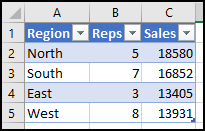
\includegraphics[width=\maxwidth{.45\linewidth}]{gfx/apa_fig01}
		\caption{AND Example Worksheet}
		\label{apa:and}
	\end{figure}

	\noindent If the following function were entered in cell $ E2 $:

	{\color{Syntax}
	\textit{\textbf{=AND(B2$>$1,B2$<$10)}}
	}

	\noindent it would return TRUE.

\end{addmargin}

\section{AVERAGE}

Returns the average (arithmetic mean) of the arguments.

\begin{addmargin}[1cm]{0cm}

	\medskip
	\underline{\textsc{Syntax:}}
	\medskip

	{\color{Syntax}
		\noindent\textbf{\textit{AVERAGE(number1, [number2], ...)}}
	}
	
	\begin{description}
		\item[Number1] \textit{Required}. The first number, cell reference, or range for which you want the average.
		\item[Number2, ...] \textit{Optional}. Additional numbers, cell references or ranges for which you want the average, up to a maximum of 255.
	\end{description}

	\medskip
	\noindent\underline{\textsc{Example:}}
	\medskip
	
	\noindent Consider the worksheet illustrated in Figure \ref{apa:avr}.

	\begin{figure}[H]
		\centering
		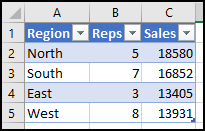
\includegraphics[width=\maxwidth{.45\linewidth}]{gfx/apa_fig01}
		\caption{AVERAGE Example Worksheet}
		\label{apa:avr}
	\end{figure}
	
	\noindent If the following function were entered in cell $ E2 $:
	
	{\color{Syntax}
		\textit{\textbf{=AVERAGE(B2:B5)}}
	}
	
	\noindent it would return $ 5.75 $.

\end{addmargin}

\section{CONCATENATE}

Joins two or more text strings into one string. \textbf{IMPORTANT}: This function was replaced with \textit{CONCAT} in Excel 365, but the syntax is the same for both functions.

\begin{addmargin}[1cm]{0cm}

	\medskip
	\underline{\textsc{Syntax:}}
	\medskip

	{\color{Syntax}
		\noindent\textbf{\textit{CONCATENATE(text1, [text2], ...)}}
	}
	
	\begin{description}
		\item[text1] \textit{Required}. The first item to join. The item can be a text value, number, or cell reference.
		\item[text2, ...] \textit{Optional}. Additional text items to join. You can have up to 255 items, up to a total of 8,192 characters.
	\end{description}

	\medskip
	\noindent\underline{\textsc{Example:}}
	\medskip
	
	\noindent Consider the worksheet illustrated in Figure \ref{apa:con}.

	\begin{figure}[H]
		\centering
		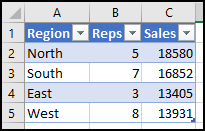
\includegraphics[width=\maxwidth{.45\linewidth}]{gfx/apa_fig01}
		\caption{CONCATENATE Example Worksheet}
		\label{apa:con}
	\end{figure}
	
	\noindent If the following function were entered in cell $ E2 $:
	
	{\color{Syntax}
		\textit{\textbf{=CONCATENATE(A2,A4)}}
	}
	
	\noindent it would return \textit{NorthEast}.
	
\end{addmargin}

\section{COUNT}

Counts the number of cells that contain numerical values. Cells with non-numeric content are ignored.

\begin{addmargin}[1cm]{0cm}

	\medskip
	\underline{\textsc{Syntax:}}
	\medskip

	{\color{Syntax}
		\noindent\textbf{\textit{COUNT(value1, [value2], ...)}}
	}
	
	\begin{description}
		\item[value1] \textit{Required}. The first item, cell reference, or range within which the cells containing numbers must be counted.
		\item[value2, ...] \textit{Optional}. Up to 255 additional items, cell references, or ranges within which the cells containing numbers must be counted.
	\end{description}

	\medskip
	\noindent\underline{\textsc{Example:}}
	\medskip
	
	\noindent Consider the worksheet illustrated in Figure \ref{apa:cnt}.

	\begin{figure}[H]
		\centering
		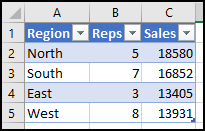
\includegraphics[width=\maxwidth{.45\linewidth}]{gfx/apa_fig01}
		\caption{COUNT Example Worksheet}
		\label{apa:cnt}
	\end{figure}
	
	\noindent If the following function were entered in cell $ E2 $:
	
	{\color{Syntax}
		\textit{\textbf{=COUNT(B2:B5)}}
	}

	\noindent it would return $ 4 $.

\end{addmargin}

\section{COUNTIF}

Counts the number of cells that meet a criterion.

\begin{addmargin}[1cm]{0cm}

	\medskip
	\underline{\textsc{Syntax:}}
	\medskip

	{\color{Syntax}
		\noindent\textbf{\textit{COUNTIF(range, criteria)}}
	}
	
	\begin{description}
		\item[range] \textit{Required}. The group of cells to count. \textit{Range} can contain numbers, arrays, a named range, or references that contain numbers. Blank and text values are ignored.
		\item[criteria] \textit{Required}. A number, expression, cell reference, or text string that determines which cells will be counted.
	\end{description}

	\medskip
	\noindent\underline{\textsc{Example:}}
	\medskip
	
	\noindent Consider the worksheet illustrated in Figure \ref{apa:cif}.

	\begin{figure}[H]
		\centering
		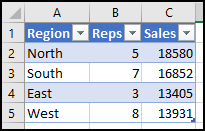
\includegraphics[width=\maxwidth{.45\linewidth}]{gfx/apa_fig01}
		\caption{COUNTIF Example Worksheet}
		\label{apa:cif}
	\end{figure}
	
	\noindent If the following function were entered in cell $ E2 $:
	
	{\color{Syntax}
		\textit{\textbf{=COUNTIF(B2:B5,''$ > $5'')}}
	}

	\noindent it would return $ 2 $.

\end{addmargin}

\section{COUNTIFS}

Applies criteria to cells across multiple ranges and counts the number of times all criteria are met.

\begin{addmargin}[1cm]{0cm}

	\medskip
	\underline{\textsc{Syntax:}}
	\medskip

	{\color{Syntax}
		\noindent\textbf{\textit{COUNTIFS(range1, criteria1, [range2, criteria2], ...)}}
	}
	
	\begin{description}
		\item[range1] \textit{Required}. The first range in which to evaluate the associated criteria.
		\item[criteria1] \textit{Required}. The criteria in the form of a number, expression, cell reference, or text string that determines which cells will be counted.
		\item[range2, criteria2, ...] \textit{Optional}. Additional ranges and criteria. Up to $ 127 $ range/criteria pairs are allowed.
	\end{description}

	\medskip
	\noindent\underline{\textsc{Example:}}
	\medskip
	
	\noindent Consider the worksheet illustrated in Figure \ref{apa:cfs}.

	\begin{figure}[H]
		\centering
		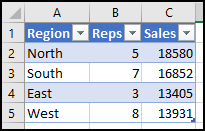
\includegraphics[width=\maxwidth{.45\linewidth}]{gfx/apa_fig01}
		\caption{COUNTIFS Example Worksheet}
		\label{apa:cfs}
	\end{figure}
	
	\noindent If the following function were entered in cell $ E2 $:
	
	{\color{Syntax}
		\textit{\textbf{=COUNTIFS(B2:B5,''$ > $3'',B2:B5,''$ < $8'')}}
	}
	
	\noindent it would return $ 2 $.

\end{addmargin}

\section{DATE}

Combines three separate values to form a date.

\begin{addmargin}[1cm]{0cm}

	\medskip
	\underline{\textsc{Syntax:}}
	\medskip

	{\color{Syntax}
		\noindent\textbf{\textit{DATE(year,month,day)}}
	}
	
	\begin{description}
		\item[year] \textit{Required}. The value of the year argument can include one to four digits. Excel interprets the year argument according to the date system the computer is using.
		\item[month] \textit{Required}. An integer representing the month of the year from $ 1 $ to $ 12 $ (January to December).
		\item[day] \textit{Required}. An integer representing the day of the month from $ 1 $ to $ 31 $.
	\end{description}

	\medskip
	\noindent\underline{\textsc{Example:}}
	\medskip
		
	\noindent If the following function were entered in cell $ A1 $:
	
	{\color{Syntax}
		\textit{\textbf{=DATE(2020,3,4)}}
	}

	\noindent it would return the date $ 3/4/2020 $ formatted according to the settings on the local computer.
	
\end{addmargin}

\section{DATEDIF}

Calculates the number of days, months, or years between two dates. \textbf{Warning}: Excel provides the \textit{DATEDIF} function in order to support older workbooks from Lotus 1-2-3. The \textit{DATEDIF} function may calculate incorrect results under certain scenarios.

\begin{addmargin}[1cm]{0cm}

	\medskip
	\underline{\textsc{Syntax:}}
	\medskip

	{\color{Syntax}
		\noindent\textbf{\textit{DATEDIF(start\_date,end\_date,unit)}}
	}
	
	\begin{description}
		\item[start\_date] \textit{Required}. A date that represents the first, or starting date of a given period. Dates may be entered as text strings within quotation marks (for example, ``1/30/2001'') or as the result of other formulas or functions.
		\item[end\_date] \textit{Required}. A date that represents the last, or ending, date of the period.
		\item[unit] \textit{Required}. The type of information to be returned. ``Y'' is the number of complete years in the period, ``M'' is the number of complete months in the period, ``D'' is the number of complete days in the period. 
	\end{description}

	\medskip
	\noindent\underline{\textsc{Example:}}
	\medskip
	
	\noindent Consider the worksheet illustrated in Figure \ref{apa:ddf}.
	
	\begin{figure}[H]
		\centering
		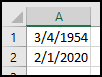
\includegraphics[width=\maxwidth{.25\linewidth}]{gfx/apa_fig02}
		\caption{DATEDIF Example Worksheet}
		\label{apa:ddf}
	\end{figure}
	
	\noindent If the following function were entered in cell $ C2 $:
	
	{\color{Syntax}
		\textit{\textbf{=DATEDIF(A1,A2,"Y")}}
	}
	
	\noindent it would return $ 65 $. This is how a person's age can be calculated with Excel.

\end{addmargin}

\section{IF}

Makes logical comparisons between a value and what was expected. This is one of the most popular Excel functions.

\begin{addmargin}[1cm]{0cm}

	\medskip
	\underline{\textsc{Syntax:}}
	\medskip

	{\color{Syntax}
		\noindent\textbf{\textit{IF(logical\_test, value\_if\_true, [value\_if\_false])}}
	}
	
	\begin{description}
		\item[logical\_test] \textit{Required}. The condition being tested.
		\item[value\_if\_true] \textit{Required}. The value returned if the result of logical\_test is TRUE.
		\item[unit] \textit{Optional}. The value returned if the result of logical\_test is FALSE. 
	\end{description}

	\medskip
	\noindent\underline{\textsc{Example:}}
	\medskip
	
	\noindent Consider the worksheet illustrated in Figure \ref{apa:if}.
	
	\begin{figure}[H]
		\centering
		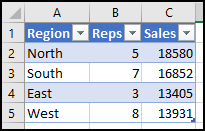
\includegraphics[width=\maxwidth{.45\linewidth}]{gfx/apa_fig01}
		\caption{IF Example Worksheet}
		\label{apa:if}
	\end{figure}
	
	\noindent If the following function were entered in cell $ E2 $:
	
	{\color{Syntax}
		\textit{\textbf{=IF(C2$ > $15000,"Bonus","Regular")}}
	}
	
	\noindent it would return \textit{Bonus}.

\end{addmargin}

\section{INDEX}

Returns a value or the reference to a value from within a table or range.

\begin{addmargin}[1cm]{0cm}
	
	\medskip
	\underline{\textsc{Syntax:}}
	\medskip
	
	{\color{Syntax}
		\noindent\textbf{\textit{INDEX(array, row\_num, [column\_num])}}
	}
	
	\begin{description}
		\item[array] \textit{Required}. A range of cells or an array constant.
		\item[row\_num] \textit{Required}, unless column\_num is present. Selects the row in \textit{array} from which to return a value. If row\_num is omitted, column\_num is required.
		\item[column\_num] \textit{Optional}. Selects the column in array from which to return a value. If column\_num is omitted, row\_num is required. 
	\end{description}

	\medskip
	\noindent\underline{\textsc{Example:}}
	\medskip
	
	\noindent Consider the worksheet illustrated in Figure \ref{apa:idx}.
	
	\begin{figure}[H]
		\centering
		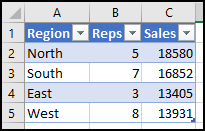
\includegraphics[width=\maxwidth{.45\linewidth}]{gfx/apa_fig01}
		\caption{INDEX Example Worksheet}
		\label{apa:idx}
	\end{figure}
	
	\noindent If the following function were entered in cell $ E2 $:
	
	{\color{Syntax}
		\textit{\textbf{=INDEX(A1:C5,4,3)}}
	}
	
	\noindent it would return $ 13405 $.

\end{addmargin}

\section{LEFT}

Returns the first character or characters in a text string, based on the number of characters specified.

\begin{addmargin}[1cm]{0cm}
	
	\medskip
	\underline{\textsc{Syntax:}}
	\medskip
	
	{\color{Syntax}
		\noindent\textbf{\textit{LEFT(text, [num\_chars])}}
	}
	
	\begin{description}
		\item[text] \textit{Required}. The text string that contains the characters to be extracted.
		\item[num\_chars] \textit{Optional}. Specifies the number of characters to be extracted. If num\_chars is omitted, it is assumed to be $ 1 $.
	\end{description}

	\medskip
	\noindent\underline{\textsc{Example:}}
	\medskip
	
	\noindent Consider the worksheet illustrated in Figure \ref{apa:lef}.
	
	\begin{figure}[H]
		\centering
		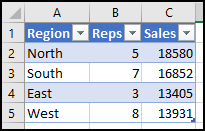
\includegraphics[width=\maxwidth{.45\linewidth}]{gfx/apa_fig01}
		\caption{LEFT Example Worksheet}
		\label{apa:lef}
	\end{figure}
	
	\noindent If the following function were entered in cell $ E2 $:
	
	{\color{Syntax}
		\textit{\textbf{=LEFT(A2,3)}}
	}
	
	\noindent it would return \textit{Nor}.

\end{addmargin}

\section{LOWER}

Converts all uppercase letters in a text string to lowercase.

\begin{addmargin}[1cm]{0cm}
	
	\medskip
	\underline{\textsc{Syntax:}}
	\medskip
	
	{\color{Syntax}
		\noindent\textbf{\textit{LOWER(text)}}
	}
	
	\begin{description}
		\item[text] \textit{Required}. The text string that contains the characters to be converted to lowercase.
	\end{description}

	\medskip
	\noindent\underline{\textsc{Example:}}
	\medskip
	
	\noindent Consider the worksheet illustrated in Figure \ref{apa:low}.
	
	\begin{figure}[H]
		\centering
		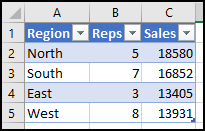
\includegraphics[width=\maxwidth{.45\linewidth}]{gfx/apa_fig01}
		\caption{LOWER Example Worksheet}
		\label{apa:low}
	\end{figure}
	
	\noindent If the following function were entered in cell $ E2 $:
	
	{\color{Syntax}
		\textit{\textbf{=LOWER(A2)}}
	}
	
	\noindent it would return \textit{north}.

\end{addmargin}

\section{MATCH}

Searches for a specified item in a range of cells and then returns the relative position of that item in the range. This function is commonly combined with \textit{Index} to lookup data in a table.

\begin{addmargin}[1cm]{0cm}
	
	\medskip
	\underline{\textsc{Syntax:}}
	\medskip
	
	{\color{Syntax}
		\noindent\textbf{\textit{MATCH(lookup\_value, lookup\_array, [match\_type])}}
	}
	
	\begin{description}
		\item[lookup\_value] \textit{Required}. The value that to be matched in \textit{lookup\_array}.
		\item[lookup\_array] \textit{Required}. The range of cells being searched.
		\item[match\_type] \textit{Optional}. The number $ -1 $, $ 0 $, or $ 1 $ specifies how Excel matches \textit{lookup\_value} with values in \textit{lookup\_array}. $ 1 $ finds the largest value that is less than or equal to \textit{lookup\_value}. $ 0 $ finds the first value that is exactly equal to \textit{lookup\_value}. $ -1 $ finds the smallest value that is greater than or equal to \textit{lookup\_value}. If omitted, the default is $ 1 $.
	\end{description}

	\medskip
	\noindent\underline{\textsc{Example:}}
	\medskip
	
	\noindent Consider the worksheet illustrated in Figure \ref{apa:mat}.
	
	\begin{figure}[H]
		\centering
		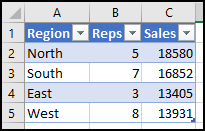
\includegraphics[width=\maxwidth{.45\linewidth}]{gfx/apa_fig01}
		\caption{MATCH Example Worksheet}
		\label{apa:mat}
	\end{figure}
	
	\noindent If the following function were entered in cell $ E2 $:
	
	{\color{Syntax}
		\textit{\textbf{=MATCH(3,B1:B5,0)}}
	}
	
	\noindent it would return $ 4 $ since the $ 3 $ is in the fourth row in \textit{Column B}.

\end{addmargin}

\section{MAX}

Returns the largest value in a set of values. 

\begin{addmargin}[1cm]{0cm}
	
	\medskip
	\underline{\textsc{Syntax:}}
	\medskip
	
	{\color{Syntax}
		\noindent\textbf{\textit{MAX(number1, [number2], ...)}}
	}
	
	\begin{description}
		\item[number1, number2, ...] \textit{Required}. Up to $ 255 $ numbers for which the maximum value is returned. This is usually a reference to a range of numbers.
	\end{description}

	\medskip
	\noindent\underline{\textsc{Example:}}
	\medskip
	
	\noindent Consider the worksheet illustrated in Figure \ref{apa:max}.
	
	\begin{figure}[H]
		\centering
		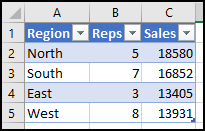
\includegraphics[width=\maxwidth{.45\linewidth}]{gfx/apa_fig01}
		\caption{MAX Example Worksheet}
		\label{apa:max}
	\end{figure}
	
	\noindent If the following function were entered in cell $ E2 $:
	
	{\color{Syntax}
		\textit{\textbf{=MAX(B1:B5)}}
	}
	
	\noindent it would return $ 18580 $.

\end{addmargin}

\section{MID}

Returns a specific number of characters from a text string, starting at the position specified, based on the number of characters specified.

\begin{addmargin}[1cm]{0cm}
	
	\medskip
	\underline{\textsc{Syntax:}}
	\medskip
	
	{\color{Syntax}
		\noindent\textbf{\textit{MID(text, start\_num, num\_chars)}}
	}
	
	\begin{description}
		\item[text] \textit{Required}. The text string that contains the characters to be extracted.
		\item[start\_num] \textit{Required}. The position of the first character to be extracted in \textit{text}. The first character in \textit{text} has a start\_num of $ 1 $, and so on.
		\item[num\_chars] \textit{Required}. Specifies the number of characters to be extracted. 
	\end{description}

	\medskip
	\noindent\underline{\textsc{Example:}}
	\medskip
	
	\noindent Consider the worksheet illustrated in Figure \ref{apa:mid}.
	
	\begin{figure}[H]
		\centering
		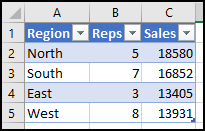
\includegraphics[width=\maxwidth{.45\linewidth}]{gfx/apa_fig01}
		\caption{MID Example Worksheet}
		\label{apa:mid}
	\end{figure}
	
	\noindent If the following function were entered in cell $ E2 $:
	
	{\color{Syntax}
		\textit{\textbf{=MID(A2,2,3)}}
	}
	
	\noindent it would return \textit{ort}.

\end{addmargin}

\section{MIN}

Returns the smallest value in a set of values. 

\begin{addmargin}[1cm]{0cm}
	
	\medskip
	\underline{\textsc{Syntax:}}
	\medskip
	
	{\color{Syntax}
		\noindent\textbf{\textit{MIN(number1, [number2], ...)}}
	}
	
	\begin{description}
		\item[number1, number2, ...] \textit{Required}. Up to $ 255 $ numbers for which the minimum value is returned.  This is usually a reference to a range of numbers.
	\end{description}

	\medskip
	\noindent\underline{\textsc{Example:}}
	\medskip
	
	\noindent Consider the worksheet illustrated in Figure \ref{apa:min}.
	
	\begin{figure}[H]
		\centering
		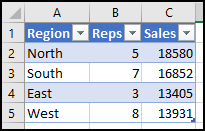
\includegraphics[width=\maxwidth{.45\linewidth}]{gfx/apa_fig01}
		\caption{MIN Example Worksheet}
		\label{apa:min}
	\end{figure}
	
	\noindent If the following function were entered in cell $ E2 $:
	
	{\color{Syntax}
		\textit{\textbf{=MIN(B1:B5)}}
	}
	
	\noindent it would return $ 13405 $.

\end{addmargin}

\section{NOW}

Returns the serial number of the current date and time. If the cell format was \textit{General} before the function was entered, Excel changes the cell format so that it matches the date and time format of the regional settings. Note: to get only the date without the time, use the \textit{TODAY} function.

\begin{addmargin}[1cm]{0cm}
	
	\medskip
	\underline{\textsc{Syntax:}}
	\medskip
	
	{\color{Syntax}
		\noindent\textbf{\textit{NOW()}}
	}
	
	\medskip
	\noindent The \textit{NOW} function has no arguments.
	
	\medskip
	\noindent\underline{\textsc{Example:}}
	\medskip
	
	\noindent If the following function were entered in cell $ A1 $:
	
	{\color{Syntax}
		\textit{\textbf{=NOW()}}
	}
	
	\noindent it would return the current date and time. When this was written the value returned was \textit{12/27/2020 12:42}.
		
\end{addmargin}

\section{NOT}

Reverses the value of its logical argument. 

\begin{addmargin}[1cm]{0cm}
	
	\medskip
	\underline{\textsc{Syntax:}}
	\medskip
	
	{\color{Syntax}
		\noindent\textbf{\textit{NOT(logical)}}
	}
	
	\begin{description}
		\item[logical] \textit{Required}. A value or expression that can be evaluated to TRUE or FALSE. If \textit{logical} is FALSE, NOT returns TRUE; if logical is TRUE, NOT returns FALSE.
	\end{description}

	\medskip
\noindent\underline{\textsc{Example:}}
\medskip

\noindent Consider the worksheet illustrated in Figure \ref{apa:not}.

\begin{figure}[H]
	\centering
	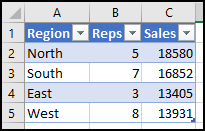
\includegraphics[width=\maxwidth{.45\linewidth}]{gfx/apa_fig01}
	\caption{NOT Example Worksheet}
	\label{apa:not}
\end{figure}

\noindent If the following function were entered in cell $ E2 $:

{\color{Syntax}
	\textit{\textbf{=NOT(B2$ > $3)}}
}

\noindent it would return FALSE. Note, $ B2 > 3 $ is TRUE, but the NOT function changes the value returned to FALSE.

\end{addmargin}

\section{OR}

Returns TRUE if any of its arguments evaluate to TRUE and FALSE if all arguments evaluate to FALSE.

\begin{addmargin}[1cm]{0cm}
	
	\medskip
	\underline{\textsc{Syntax:}}
	\medskip
	
	{\color{Syntax}
		\noindent\textit{\textbf{OR(logical1, [logical2], ...)}}
	}
	
	\begin{description}
		\item[Logical1] \textit{Required}. The first condition to be tested that can evaluate to either TRUE or FALSE.
		\item[Logical2, ...] \textit{Optional}. Additional conditions to be tested that can evaluate to either TRUE or FALSE, up to a maximum of 255 conditions.
	\end{description}

	\medskip
	\noindent\underline{\textsc{Example:}}
	\medskip
	
	\noindent Consider the worksheet illustrated in Figure \ref{apa:or}.
	
	\begin{figure}[H]
		\centering
		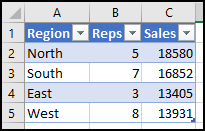
\includegraphics[width=\maxwidth{.45\linewidth}]{gfx/apa_fig01}
		\caption{OR Example Worksheet}
		\label{apa:or}
	\end{figure}
	
	\noindent If the following function were entered in cell $ E2 $:
	
	{\color{Syntax}
		\textit{\textbf{=OR(B2$>$1,B2$<$10)}}
	}
	
	\noindent it would return TRUE.

\end{addmargin}

\section{PMT}

Calculates the payment for a loan based on constant payments and a constant interest rate.

\begin{addmargin}[1cm]{0cm}
	
	\medskip
	\underline{\textsc{Syntax:}}
	\medskip
	
	{\color{Syntax}
		\noindent\textit{\textbf{PMT(rate, nper, pv, [fv], [type])}}
	}
	
	\begin{description}
		\item[rate] \textit{Required}. The interest rate for the loan.
		\item[nper] \textit{Required}. The total number of payments for the loan.
		\item[pv] \textit{Required}. The present value, or the total amount that a series of future payments is worth now; also known as the principal.
		\item[fv] \textit{Optional}. The future value, or a cash balance attained after the last payment is made. If \textit{fv} is omitted, it is assumed to be $ 0 $.  
		\item[type] \textit{Optional}. Indicates when payments are due, $ 0 $ for the end of the period or $ 1 $ for the beginning of the period.
	\end{description}

	\medskip
	\noindent\underline{\textsc{Example:}}
	\medskip
	
	\noindent If the following function were entered in cell $ A1 $:
	
	{\color{Syntax}
		\textit{\textbf{=PMT(0.05/12,5*12,-25000)}}
	}
	
	\noindent it would return $ 471.78 $. So, a loan of \$$ 25000 $ at $ 5 $\% interest rate per year for a term of $ 5 $ years would generate a monthly payment of $ 471.78 $.

\end{addmargin}

\section{PROPER}

Capitalizes the first letter in a text string and any other letters in text that follow any character other than a letter. Converts all other letters to lowercase letters.

\begin{addmargin}[1cm]{0cm}
	
	\medskip
	\underline{\textsc{Syntax:}}
	\medskip
	
	{\color{Syntax}
		\noindent\textbf{\textit{PROPER(text)}}
	}
	
	\begin{description}
		\item[text] \textit{Required}. The text string that contains the characters to be partially capitalized.
	\end{description}

	\medskip
	\noindent\underline{\textsc{Example:}}
	\medskip
	
	\noindent Consider the worksheet illustrated in Figure \ref{apa:pro}.
	
	\begin{figure}[H]
		\centering
		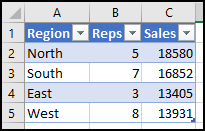
\includegraphics[width=\maxwidth{.45\linewidth}]{gfx/apa_fig01}
		\caption{PROPER Example Worksheet}
		\label{apa:pro}
	\end{figure}
	
	\noindent If the following function were entered in cell $ E2 $:
	
	{\color{Syntax}
		\textit{\textbf{=PROPER(A2)}}
	}
	
	\noindent it would return \textit{North}.

\end{addmargin}

\section{RANDBETWEEN}

Returns a random integer number between the numbers specified. A new random integer number is returned every time the worksheet is calculated.

\begin{addmargin}[1cm]{0cm}
	
	\medskip
	\underline{\textsc{Syntax:}}
	\medskip
	
	{\color{Syntax}
		\noindent\textbf{\textit{RANDBETWEEN(bottom, top)}}
	}
	
	\begin{description}
		\item[bottom] \textit{Required}. The smallest integer to be returned.
		\item[top] \textit{Required}. The largest integer to be returned.
	\end{description}

	\medskip
	\noindent\underline{\textsc{Example:}}
	\medskip
	
	\noindent If the following function were entered in cell $ A1 $:
	
	{\color{Syntax}
		\textit{\textbf{=RANDBETWEEN(10,99)}}
	}
	
	\noindent it would return a random integer between $ 10 $ and $ 99 $ (inclusive).

\end{addmargin}

\section{RIGHT}

Returns the last character or characters in a text string, based on the number of characters specified.

\begin{addmargin}[1cm]{0cm}
	
	\medskip
	\underline{\textsc{Syntax:}}
	\medskip
	
	{\color{Syntax}
		\noindent\textbf{\textit{RIGHT(text, [num\_chars])}}
	}
	
	\begin{description}
		\item[text] \textit{Required}. The text string that contains the characters to be extracted.
		\item[num\_chars] \textit{Optional}. Specifies the number of characters to be extracted. If \textit{num\_chars} is omitted, it is assumed to be $ 1 $.
	\end{description}

	\medskip
	\noindent\underline{\textsc{Example:}}
	\medskip
	
	\noindent Consider the worksheet illustrated in Figure \ref{apa:rig}.
	
	\begin{figure}[H]
		\centering
		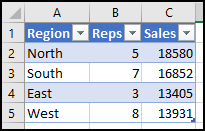
\includegraphics[width=\maxwidth{.45\linewidth}]{gfx/apa_fig01}
		\caption{RIGHT Example Worksheet}
		\label{apa:rig}
	\end{figure}
	
	\noindent If the following function were entered in cell $ E2 $:
	
	{\color{Syntax}
		\textit{\textbf{=RIGHT(A2,3)}}
	}
	
	\noindent it would return \textit{rth}.

\end{addmargin}

\section{ROUND}

Rounds a number to a specified number of digits.  

\begin{addmargin}[1cm]{0cm}
	
	\medskip
	\underline{\textsc{Syntax:}}
	\medskip
	
	{\color{Syntax}
		\noindent\textbf{\textit{ROUND(number, num\_digits)}}
	}
	
	\begin{description}
		\item[number] \textit{Required}. The number to be rounded.
		\item[num\_digits] \textit{Required}. The number of digits to which \textit{number} is rounded. If \textit{num\_digits} is greater than $ 0 $ then number is rounded to the specified number of decimal places. If \textit{num\_digits} is $ 0 $ the number is rounded to the nearest integer. If \textit{num\_digits} is less than $ 0 $, the number is rounded to the left of the decimal point.
	\end{description}

	\medskip
	\noindent\underline{\textsc{Example:}}
	\medskip
	
	\noindent Consider the worksheet illustrated in Figure \ref{apa:ron}.
	
	\begin{figure}[H]
		\centering
		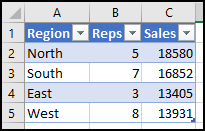
\includegraphics[width=\maxwidth{.45\linewidth}]{gfx/apa_fig01}
		\caption{ROUND Example Worksheet}
		\label{apa:ron}
	\end{figure}
	
	\noindent If the following function were entered in cell $ E2 $:
	
	{\color{Syntax}
		\textit{\textbf{=ROUND(C5,-2)}}
	}
	
	\noindent it would return $ 13900 $.

\end{addmargin}

\section{SEARCH}

Returns the location of one text string inside another.

\begin{addmargin}[1cm]{0cm}
	
	\medskip
	\underline{\textsc{Syntax:}}
	\medskip
	
	{\color{Syntax}
		\noindent\textbf{\textit{SEARCH(find\_text, within\_text, [start\_num])}}
	}
	
	\begin{description}
		\item[find\_text] \textit{Required}. The text to be found.
		\item[within\_text] \textit{Required}. The text to be searched.
		\item[start\_num] \textit{Optional}. Starting position in the text to be searched. This defaults to $ 1 $.
	\end{description}

	\medskip
	\noindent\underline{\textsc{Example:}}
	\medskip
	
	\noindent If the following function were entered in cell $ A1 $:
	
	{\color{Syntax}
		\textit{\textbf{=SEARCH("or","horse")}}
	}
	
	\noindent it would return $ 2 $ since the word \textit{or} starts at position $ 2 $ in \textit{horse}.

\end{addmargin}

\section{SUM}

Sums the values in a range.

\begin{addmargin}[1cm]{0cm}
	
	\medskip
	\underline{\textsc{Syntax:}}
	\medskip
	
	{\color{Syntax}
		\noindent\textbf{\textit{SUM(number1,[number2],...)}}
	}
	
	\begin{description}
		\item[number1] \textit{Required}. The first number to be added.
		\item[number2, ...] \textit{Optional}. Up to 255 additional numbers to be added.
	\end{description}

	\medskip
	\noindent\underline{\textsc{Example:}}
	\medskip
	
	\noindent Consider the worksheet illustrated in Figure \ref{apa:sum}.
	
	\begin{figure}[H]
		\centering
		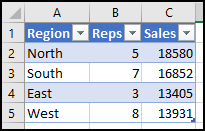
\includegraphics[width=\maxwidth{.45\linewidth}]{gfx/apa_fig01}
		\caption{SUM Example Worksheet}
		\label{apa:sum}
	\end{figure}
	
	\noindent If the following function were entered in cell $ E2 $:
	
	{\color{Syntax}
		\textit{\textbf{=SUM(B1:B5)}}
	}
	
	\noindent it would return $ 23 $.

\end{addmargin}

\section{SUMIF}

Sums the values in a range that meet a specified criteria. 

\begin{addmargin}[1cm]{0cm}
	
	\medskip
	\underline{\textsc{Syntax:}}
	\medskip
	
	{\color{Syntax}
		\noindent\textbf{\textit{SUMIF(range, criteria, [sum\_range])}}
	}
	
	\begin{description}
		\item[range] \textit{Required}. The range of cells to be evaluated by criteria. 
		\item[criteria] \textit{Required}. The criteria in the form of a number, expression, a cell reference, text, or a function that defines which cells will be added.
		\item[sum\_range] \textit{Optional}. The actual cells to add if cells other than those specified in the range argument are to be added. If the \textit{sum\_range} argument is omitted, Excel adds the cells that are specified in the \textit{range} argument (the same cells to which the criteria is applied).
	\end{description}

	\medskip
	\noindent\underline{\textsc{Example:}}
	\medskip
	
	\noindent Consider the worksheet illustrated in Figure \ref{apa:sif}.
	
	\begin{figure}[H]
		\centering
		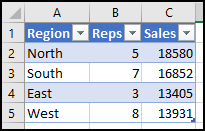
\includegraphics[width=\maxwidth{.45\linewidth}]{gfx/apa_fig01}
		\caption{SUMIF Example Worksheet}
		\label{apa:sif}
	\end{figure}
	
	\noindent If the following function were entered in cell $ E2 $:
	
	{\color{Syntax}
		\textit{\textbf{=SUMIF(B2:B5,"$ > $5")}}
	}
	
	\noindent it would return $ 15 $, which is the sum of $ 7 $ and $ 8 $.

\end{addmargin}

\section{SUMIFS}

Sums the values in a range that meet multiple specified criteria.

\begin{addmargin}[1cm]{0cm}
	
	\medskip
	\underline{\textsc{Syntax:}}
	\medskip
	
	{\color{Syntax}
		\noindent\textbf{\textit{SUMIFS(range, crit\_range1, crit1, [crit\_range2, crit2], ...)}}
	}
	
	\begin{description}
		\item[range] \textit{Required}. The range of cells to be summed. 
		\item[crit\_range1] \textit{Required}. The range that is tested using \textit{crit1}.
		\item[crit1] \textit{Required}. The criteria that defines which cells in \textit{crit\_range1} will be added.
		\item[crit\_range2, crit2, ...] \textit{Optional}. Additional ranges and their associated criteria. Up to 127 range/criteria pairs can be entered.
	\end{description}

	\medskip
	\noindent\underline{\textsc{Example:}}
	\medskip
	
	\noindent Consider the worksheet illustrated in Figure \ref{apa:sfs}.
	
	\begin{figure}[H]
		\centering
		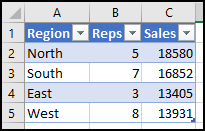
\includegraphics[width=\maxwidth{.45\linewidth}]{gfx/apa_fig01}
		\caption{SUMIFS Example Worksheet}
		\label{apa:sfs}
	\end{figure}
	
	\noindent If the following function were entered in cell $ E2 $:
	
	{\color{Syntax}
		\textit{\textbf{=SUMIFS(B2:B5,B2:B5,"$ > $3",B2:B5,"$ < $8")}}
	}
	
	\noindent it would return $ 12 $, which is the sum of $ 5 $ and $ 7 $.

\end{addmargin}
 
\section{TODAY}

Returns the serial number of the current date. If the cell format was \textit{General} before the function was entered, Excel changes the cell format so that it matches the date and time format of the regional settings. Note: to get both the date and time, use the \textit{NOW} function.

\begin{addmargin}[1cm]{0cm}
	
	\medskip
	\underline{\textsc{Syntax:}}
	\medskip
	
	{\color{Syntax}
		\noindent\textbf{\textit{TODAY()}}
	}
	
	\medskip
	\noindent The \textit{TODAY} function has no arguments.
	
	\medskip
	\noindent\underline{\textsc{Example:}}
	\medskip
	
	\noindent If the following function were entered in cell A1:
	
	{\color{Syntax}
		\textit{\textbf{=TODAY()}}
	}
	
	\noindent it would return the current date. When this was written the value returned was \textit{12/27/2020}.
	
	
\end{addmargin}

\section{TRIM}

Removes all spaces from text except for single spaces between words. 

\begin{addmargin}[1cm]{0cm}
	
	\medskip
	\underline{\textsc{Syntax:}}
	\medskip
	
	{\color{Syntax}
		\noindent\textbf{\textit{TRIM(text)}}
	}
	
	\begin{description}
		\item[text] \textit{Required}. The text from which excess spaces should be removed.
	\end{description}

	\medskip
	\noindent\underline{\textsc{Example:}}
	\medskip
	
	\noindent If the following function were entered in cell $ A1 $:
	
	{\color{Syntax}
		\textit{\textbf{=TRIM(``\:\:\:Two\:\:\:\:\:Spaces\:\:\:\:")}}
	}
	
	\noindent it would return \textit{Two Spaces}.

\end{addmargin}

\section{UPPER}

Converts all lowercase letters in a text string to uppercase.

\begin{addmargin}[1cm]{0cm}
	
	\medskip
	\underline{\textsc{Syntax:}}
	\medskip
	
	{\color{Syntax}
		\noindent\textbf{\textit{UPPER(text)}}
	}
	
	\begin{description}
		\item[text] \textit{Required}. The text string that contains the characters to be converted to uppercase.
	\end{description}

	\medskip
	\noindent\underline{\textsc{Example:}}
	\medskip
	
	\noindent Consider the worksheet illustrated in Figure \ref{apa:up}.
	
	\begin{figure}[H]
		\centering
		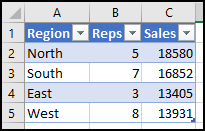
\includegraphics[width=\maxwidth{.45\linewidth}]{gfx/apa_fig01}
		\caption{UPPER Example Worksheet}
		\label{apa:up}
	\end{figure}
	
	\noindent If the following function were entered in cell $ E2 $:
	
	{\color{Syntax}
		\textit{\textbf{=UPPER(A2)}}
	}
	
	\noindent it would return \textit{NORTH}.

\end{addmargin}

\section{VLOOKUP}

Looks up a value in a table or range by row. 

\begin{addmargin}[1cm]{0cm}
	
	\medskip
	\underline{\textsc{Syntax:}}
	\medskip
	
	{\color{Syntax}
		\noindent\textbf{\textit{VLOOKUP(value, array, col\_num, [range\_lookup])}}
	}
	
	\begin{description}
		\item[value] \textit{Required}. The value to be looked up.
		\item[array] \textit{Required}. A range of cells to be searched for the \textit{value}.
		\item[col\_num] \textit{Required}. Selects the column in \textit{array} from which to return a value. The columns are numbered starting with $ 1 $ which is the far left column. 
		\item[range\_lookup] \textit{Optional}. Specifies whether an approximate match, TRUE, or exact match, FALSE, is desired. The default is approximate.
	\end{description}

	\medskip
	\noindent\underline{\textsc{Example:}}
	\medskip
	
	\noindent Consider the worksheet illustrated in Figure \ref{apa:vlk}.
	
	\begin{figure}[H]
		\centering
		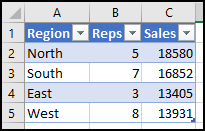
\includegraphics[width=\maxwidth{.45\linewidth}]{gfx/apa_fig01}
		\caption{VLOOKUP Example Worksheet}
		\label{apa:vlk}
	\end{figure}
	
	\noindent If the following function were entered in cell $ E2 $:
	
	{\color{Syntax}
		\textit{\textbf{=VLOOKUP(7,B2:C5,2)}}
	}
	
	\noindent it would return $ 16852 $.

\end{addmargin}


%*****************************************************
%***  Appendix B
%*****************************************************

%********************************************************************
% All about dynamic arrays in Excel 365
%*******************************************************

\chapter{Dynamic Arrays}\label{app02:dynamic}

\fmtNewExcel{Excel 365} NOTE: This appendix concerns \textit{dynamic arrays}, a feature that was first included in Excel 365 and is only available in versions of Excel that are included with a Microsoft Office subscription. Therefore, students who are using Excel 2016 will not be able to use the information in this appendix.

\section{Definition}

Dynamic arrays are grids of data created by calculating values based on the formula in a single cell. From its inception, Excel has always used a ``one cell, one formula'' approach, so designers who wanted to fill a grid of values would have to copy/paste a formula into each cell in that grid. This was time consuming and error-prone. Dynamic arrays, though, use a formula in a single cell to calculate values in many other cells, saving time and improving accuracy.

The introduction of dynamic arrays includes several new functions that make working with a data array easier. As an example, UNIQUE() will search an array and return only the unique (non-repeating) values. Additionally, dynamic array functions are automatically updated if items are added or removed from the data array.

These concepts are easiest to understand with examples.

\begin{enumbox}
	\begin{enumerate}
		\item Click \fmtButton{File $ \Rightarrow $ Open $ \Rightarrow $ Browse}.
		\item Navigate to \fmtWorksheet{APA-Data} and click \fmtButton{Open}.
		\item Click \fmtButton{File $ \Rightarrow $ Save As $ \Rightarrow $ Browse}.
		\item Navigate to the desired file location and save it with the name \fmtWorksheet{APA-Dynamic}.
		\item Click the \fmtWorksheet{Sales} worksheet tab to open the worksheet.
	\end{enumerate}
\end{enumbox}

This simple worksheet lists the names, regions, and number of monthly units sold for several sales representatives in a company. 

\section{Functions}

\subsection{Sort()}

\[ =SORT(array,[sort\_index],[sort\_order],[by\_col]) \]

One of the simplest dynamic array functions is \textit{SORT()}. The syntax above indicates that the only required variable is the array to be sorted, the others are optional. The following steps use the function in its simplest form.

\begin{enumbox}
	\begin{enumerate}
		\item Click \fmtLoc{E1} and enter \fmtTyping{Sort}.
		\item Click \fmtLoc{E2} to activate that cell.
		\item Since the array is in a named table, a column can be sorted by entering the names of the table and column, like \fmtTyping{=SORT(Sales[Name])}. Alternatively, the cell range for the Name column can be entered, \fmtTyping{=SORT(A2:A21)}, but using the table and column names is a better option since those would still be accurate if the table is later modified.
	\end{enumerate}
\end{enumbox}

Notice that even though the formula was only entered in one cell, $ E2 $, it filled an entire range, $ E2 $ : $ E21 $ with the sorted data. The sorted data is dynamic so if any of the names in \textit{Column A} are changed the list in \textit{Column E} is updated to reflect that change.

\begin{enumbox}
	\begin{enumerate}
		\item Click \fmtLoc{A14} to activate that cell.
		\item Type \fmtTyping{Alvin} to change the name \textit{Avye}.
		\item Notice that the list of names in \fmtLoc{Column E} is automatically updated so \fmtLoc{E4} contains the changed value, \textit{Alvin}, and the previous value, \textit{Avye}, is gone.
		\item Click cell \fmtLoc{A12} to activate that cell.
		\item Click \fmtButton{Home $ \Rightarrow $ Cells $ \Rightarrow $ Delete $ \Rightarrow $ Delete Table Rows}.
		\item The name \textit{Aidan} has been deleted and the list of names in \fmtLoc{Column E} is automatically updated to reflect the missing row.
		\item Click cell \fmtLoc{A13} to activate that cell.
		\item Click \fmtButton{Home $ \Rightarrow $ Cells $ \Rightarrow $ Insert $ \Rightarrow $ Insert Table Rows Above}.
		\item Click cell \fmtLoc{A12} to activate that cell.
		\item Type \fmtTyping{Bosley} then press \fmtKeystroke{Tab}.
		\item Type \fmtTyping{Northeast} then press \fmtKeystroke{Tab}.
		\item Type \fmtTyping{146} then press \fmtKeystroke{Enter}.		
		\item The name \textit{Bosley} has been added and the list of names in \fmtLoc{Column E} is automatically updated to reflect the new row.
	\end{enumerate}
\end{enumbox}

\begin{figure}[H]
	\centering
	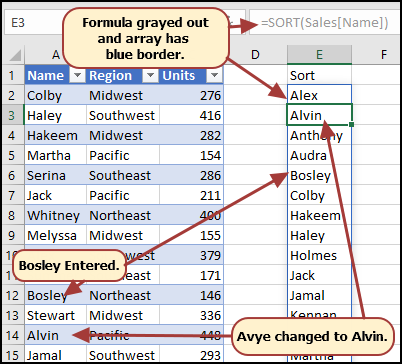
\includegraphics[width=\maxwidth{.95\linewidth}]{gfx/apb_fig01}
	\caption{Sort Array}
	\label{apb:fig01}
\end{figure}

Click in $ E2 $ and notice that the formula displayed in the formula bar is in normal font. Then click in $ E3 $ and notice that the formula displayed in the formula bar is grayed out and cannot be edited. Also notice that the range $ E2 $:$ E21 $ is surrounded with a blue border, indicating that this is a \textit{spilled array} that is generated automatically from the formula in cell $ E2 $.

\begin{center}
	\begin{infobox}{Best Practice}
		\textbf{Array Data}
		\\
		\\
		In general, it is best to keep the data referenced by a dynamic array in a data table with at least one column or one row of separation between the data table and a dynamic array. The data table can be in a different worksheet but must be in the same workbook as the dynamic array.
	\end{infobox}
\end{center}

\subsection{Sortby()}

\[ =SORTBY(array, array1, [order1], [array2, order2],…)  \]

\textit{SORTBY()} makes it possible to sort one range by another range for more complex sorts. As an example, the following steps sorts the \textit{Sales} table by \textit{Name} and \textit{Region}. 

\begin{enumbox}
	\begin{enumerate}
		\item Click \fmtLoc{F1} and enter \fmtTyping{Sortby}.
		\item Click \fmtLoc{F2} and enter\\ \fmtTyping{=SORTBY(Sales[[Name]:[Region]],Sales[Region],1, Sales[Name],1)
		}. 
	\end{enumerate}
\end{enumbox}

\begin{figure}[H]
	\centering
	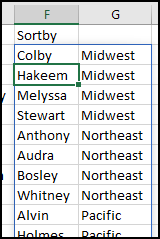
\includegraphics{gfx/apb_fig02}
	\caption{Sortby Array}
	\label{apb:fig02}
\end{figure}

\textit{Columns F:G} now contains all of the names sorted alphabetically by region. The \textit{SORTBY()} function used in $ F2 $ looks complex, but it is not that difficult to understand. Each of the sections of the command are separated by commas and described below.

\begin{description}
	\item[{Sales[[Name]:[Region]]}] \textemdash\: Sort the data in the \textit{Name} and \textit{Region} columns from the \textit{Sales} table.
	\item[{Sales[Region]}] \textemdash\: Use the \textit{Region} column as the primary sort field.
	\item[1] \textemdash\: Sort the regions alphabetically from first to last.
	\item[{Sales[Name]}] Use the \textit{Name} column as the secondary sort field; that is, sort the names alphabetically within the regions.
	\item[1] \textemdash\: Sort the names alphabetically from first to last.	
\end{description}

The \textit{SORTBY()} function is very powerful and even permits sorting by columns that are not in the final output array. For example, to sort the array in $ F2 $:$ G21 $ by \textit{Units}, change the function in $ F2 $ to:\\ \textit{=SORTBY(Sales[[Name]:[Region]], Sales[Region], 1, Sales[Units], -1)}. With this new sort order, Stewart becomes the first name in the Midwest region since he sold the most number of units in that region.

\subsection{Unique()}

\[ =UNIQUE(array,[col],[once]) \]

Follow these steps to find the unique values in a column of data.

\begin{enumbox}
	\begin{enumerate}
		\item Click \fmtLoc{H1} and enter \fmtTyping{Unique}.
		\item Click \fmtLoc{H2} and enter \fmtTyping{=UNIQUE(Sales[Region])}. 
	\end{enumerate}
\end{enumbox}

\begin{figure}[H]
	\centering
	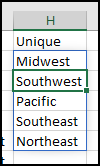
\includegraphics{gfx/apb_fig03}
	\caption{Unique Regions}
	\label{apb:fig03}
\end{figure}

Cells $ H2 $:$ H6 $ contains the unique values found in the \textit{Region} column. Complete the following steps to test the dynamic characteristic of \textit{Column H}.

\begin{enumbox}
	\begin{enumerate}
		\item Click \fmtLoc{B5} and enter \fmtTyping{Mountain}.
		\item Notice that the dynamic range \fmtLoc{H2:H7} is updated to include the new \textit{Mountain} region. 
		\item Click \fmtLoc{B5} and enter \fmtTyping{Pacific}, which was the original value.
		\item Notice that the dynamic range \fmtLoc{H2:H7} is updated to exclude the \textit{Mountain} region.		
	\end{enumerate}
\end{enumbox}

\subsection{Nesting Functions}

Dynamic array functions, like any functions, can be nested to improve their usefulness. The unique regions in \textit{Column H} would be more useful if they were in alphabetical order.

\begin{enumbox}
	\begin{enumerate}
		\item Click \fmtLoc{H2} and change the formula in that cell to \fmtTyping{=SORT(UNIQUE(Sales[Region]))}.
	\end{enumerate}
\end{enumbox}

Now the list of regions in \textit{Column H} will be sorted in alphabetical order.

\subsection{Filter()}

\[ =FILTER(array,include,[if\_empty]) \]

Dynamic arrays can be filtered to focus on specific items. The following steps remove all regions except Pacific.

\begin{enumbox}
	\begin{enumerate}
		\item Click \fmtLoc{I1} and enter \fmtTyping{Filter}.
		\item Click \fmtLoc{I2} and enter\\ \fmtTyping{=FILTER(Sales[Name],Sales[Region]=''Pacific'')}. 
	\end{enumerate}
\end{enumbox}

A dynamic array is created in $ I2 $:$ I5 $ that lists the names of everyone assigned to the Pacific region. This list would be more useful if it were alphabetized so a \textit{SORT()} function can be added. 

\begin{enumbox}
	\begin{enumerate}
		\item Click \fmtLoc{I2} and change the formula in that cell to \fmtTyping{=SORT(FILTER(Sales[Name],Sales[Region]=''Pacific''))}. 
	\end{enumerate}
\end{enumbox}

Follow these steps to test the dynamic filter.

\begin{enumbox}
	\begin{enumerate}
		\item Click \fmtLoc{B2} and enter \fmtTyping{Pacific}.
		\item Notice that \textit{Colby} is now in the \textit{Filter} list in \fmtLoc{Column I}.
		\item Click \fmtLoc{B2} and enter \fmtTyping{Midwest} to return this cell to its original value.
		\item Notice that \textit{Colby} is no longer in the \textit{Filter} list in \fmtLoc{Column I}.
	\end{enumerate}
\end{enumbox}

\subsection{Referencing A Dynamic Array}

Dynamic arrays can grow or shrink depending on the data being analyzed but formulas that refer to that array need to work, no matter its size. To do that, add a hash (\fmtKeystroke{\#}) after the array reference. This is illustrated in the following steps.

\begin{enumbox}
	\begin{enumerate}
		\item Click \fmtLoc{J1} and enter \fmtTyping{Pacific Reps}.
		\item Click \fmtLoc{J2} and enter \fmtTyping{=COUNTA(I2\#)}.
	\end{enumerate}
\end{enumbox}

\begin{figure}[H]
	\centering
	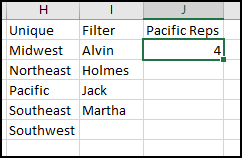
\includegraphics[width=\maxwidth{.50\linewidth}]{gfx/apb_fig04}
	\caption{Referring to a Dynamic Array}
	\label{apb:fig04}
\end{figure}

Cell $ J2 $ displays $ 4 $ since there are four representatives listed in the dynamic array starting in $ I2 $. Complete the following steps to test the dynamic charactistics of this array.

\begin{enumbox}
	\begin{enumerate}
		\item Click \fmtLoc{B2} and enter \fmtTyping{Pacific}.
		\item Notice that \textit{Colby} is now in the \textit{Filter} list in \fmtLoc{Column I} and the number of representatives in \fmtLoc{J2} has changed to $ 5 $.
		\item Click \fmtLoc{B2} and enter \fmtTyping{Midwest} to return this cell to its original value.
		\item Notice that \textit{Colby} is no longer in the \textit{Filter} list in \fmtLoc{Column I} and the number of representatives in \fmtLoc{J2} has returned to $ 4 $.
	\end{enumerate}
\end{enumbox}

The formula in cell $ J2 $ counts all of the lines in the dynamic array starting in $ I2 $ no matter how long that array grows.

\subsection{Xlookup()}

\[ =XLOOKUP(value, array, return, [not\_found], [match], [search]) \]

\textit{XLookup} is a modern and flexible replacement for older functions like \textit{VLOOKUP}, \textit{HLOOKUP}, and \textit{LOOKUP}. Complete the following steps to explore this powerful function.

\begin{enumbox}
	\begin{enumerate}
		\item Click \fmtLoc{K1} and enter \fmtTyping{XLookup}.
		\item Click \fmtLoc{K2} and enter \fmtTyping{Colby}
		\item Click \fmtLoc{L2} and enter \\ \fmtTyping{=XLOOKUP(K2,Sales[Name],Sales[[Region]:[Units]])}.
	\end{enumerate}
\end{enumbox}

\begin{figure}[H]
	\centering
	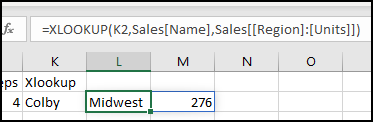
\includegraphics[width=\maxwidth{.75\linewidth}]{gfx/apb_fig05}
	\caption{XLookup Function}
	\label{apb:fig05}
\end{figure}

The \textit{XLookup} function searches in the \textit{Name} column for the name found in cell $ K2 $. When it finds that value, it returns the \textit{Region} and \textit{Units} values for that name. In the example above, \textit{Colby} returns \textit{Midwest} and $ 276 $ from the \textit{Sales} table. One of the strengths of using dynamic arrays is that if the \textit{Sales} table is modified by adding or deleting rows or columns, the \textit{XLookup} function will continue to work.

\subsection{XMatch()}

\[ =XMATCH(value, array, [match], [search]) \]

\textit{XMatch} is a modern and flexible replacement for the older \textit{MATCH} function. It performs a lookup and returns a position in vertical or horizontal ranges. Complete the following steps to explore this powerful function.

\begin{enumbox}
	\begin{enumerate}
		\item Click \fmtLoc{K4} and enter \fmtTyping{XMatch}.
		\item Click \fmtLoc{K5} and enter \fmtTyping{Colby}
		\item Click \fmtLoc{L5} and enter \\ \fmtTyping{=XMATCH(K5,Sales[Name])}.
	\end{enumerate}
\end{enumbox}

\begin{figure}[H]
	\centering
	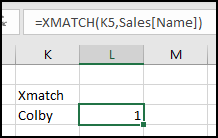
\includegraphics[width=\maxwidth{.50\linewidth}]{gfx/apb_fig06}
	\caption{XMatch Function}
	\label{apb:fig06}
\end{figure}

Cell $ L5 $ will display $ 1 $ since the value in $ K5 $, \textit{Colby}, is in row one of the \textit{Sales} table. By itself, this is of limited value, but combining \textit{XMatch} with \textit{Index} creates a powerful lookup function that can return the value in any column for any found row in a data table.

\begin{enumbox}
	\begin{enumerate}
		\item Click \fmtLoc{K7} and enter \fmtTyping{XMatch+Index}.
		\item Click \fmtLoc{K5} and enter \fmtTyping{Colby}
		\item Click \fmtLoc{L5} and enter \\ \fmtTyping{=INDEX(Sales,XMATCH(K8,Sales[Name]),3)}.
	\end{enumerate}
\end{enumbox}

\begin{figure}[H]
	\centering
	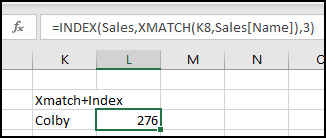
\includegraphics[width=\maxwidth{.65\linewidth}]{gfx/apb_fig07}
	\caption{XMatch+Index Function}
	\label{apb:fig07}
\end{figure}

This returns $ 276 $, which is how many units Colby sold. If the data table contained dozens of columns and hundreds of rows, \textit{XMatch+Index} is very useful in pinpointing the specific data needed.

\subsection{Randarray()}

\[ =RANDARRAY([rows],[columns],[min],[max],[whole\_number]) \]

Use the following steps to create a dynamic array of random numbers.

\begin{enumbox}
	\begin{enumerate}
		\item Click \fmtLoc{D24} and enter \fmtTyping{Random}.
		\item Click \fmtLoc{D25} and enter \fmtTyping{=RANDARRAY(3,4,10,99,TRUE)}
	\end{enumerate}
\end{enumbox}

\begin{figure}[H]
	\centering
	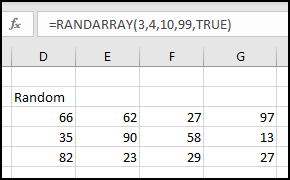
\includegraphics[width=\maxwidth{.65\linewidth}]{gfx/apb_fig08}
	\caption{Random Array}
	\label{apb:fig08}
\end{figure}

This creates an array of three rows and four columns that contain random numbers between $ 10 $ and $ 99 $. The final \textit{TRUE} restricts the random numbers to integers rather than decimals. NOTE: The function creates an array of random numbers so the illustration in this book will not match the student's work.

\subsection{Sequence()}

\[ =SEQUENCE(rows,[columns],[start],[step]) \]

Follow these steps to create a dynamic array that contains a sequence of numbers.

\begin{enumbox}
	\begin{enumerate}
		\item Click \fmtLoc{D29} and enter \fmtTyping{Sequence}.
		\item Click \fmtLoc{D30} and enter \fmtTyping{=SEQUENCE(5,3,25,3)}
	\end{enumerate}
\end{enumbox}

\begin{figure}[H]
	\centering
	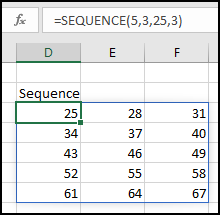
\includegraphics[width=\maxwidth{.45\linewidth}]{gfx/apb_fig09}
	\caption{Sequence}
	\label{apb:fig09}
\end{figure}

This creates a sequence of numbers filling five rows and three columns starting at $ 25 $ and stepping by $ 3 $. 

